\documentclass[twoside]{article}
\input{ISC18-english.sty}
%%%%%%%%%%%%%%%%%%%%%%%%%%%%  Make sure to compile twice for proper cross-references. %%%%%%%%%%%%%%%%%%%%%%%
%%%%%%% For proper display of references, compile the document twice. %%%%%%%%%%%%%%%%%%%%% 
%%%%%%%%%%%%%%% If using TeX Live, compile using pdflatex command %%%%%%%%%%%%%%%%%%%%%%%
\begin{document}
\thispagestyle{empty}
%%%%%%%%%%%%%%%%% Article title header  %%%%%%%%%%%%%%%%%%%%
\fancyhead[LE]{Bayesian Inference for VAR-GoGARCH Models}
%%%%%%%%%%%%%%%%% Article authors header   %%%%%%%%%%%%%%%%%%%%
\fancyhead[RO]{Manouchehri et al.}
\begin{center}
{
\includegraphics [height=25mm, width=150.3mm] {Images/isc18E}} \\
\vspace*{-1.8cm}
%\begin{center}
%\color{blue} 
%{\hspace{0.1cm}\rule{\textwidth}{1mm}}\\
%\end{center}
\vspace*{4cm}
%%%%%%%%%%%%%%%%% Article title  %%%%%%%%%%%%%%%%%%%%
{\Large \bf Bayesian Inference for VAR-GoGARCH Models under Gaussian and Skew-Normal Innovations}\\
%%%%%%%%%%%%%%%%% Article authors and affiliations %%%%%%%%%%%%%%%%%%%%
{\bf
T. Manouchehri{\footnote[1]{{\bf Corresponding Author:} {\tt t.manouchehri@shirazu.ac.ir}}, A. R. Nematollahi$^1$ , M. Sadeghi Kahmini$^1$} \\
$^1$Department of Statistics, Shiraz University, Shiraz, Iran.}
\end{center}
\rule{\textwidth}{0.2mm}\\
%%%%%%%%%%%%%%%%% Article abstract  %%%%%%%%%%%%%%%%%%%%
\noindent{\bf Abstract:}\\

Modeling multivariate financial time series requires flexible frameworks capable of capturing dynamic dependence, conditional heteroscedasticity, and asymmetric innovation distributions. This paper develops a Bayesian estimation framework for VAR-GoGARCH models under both Gaussian and skew-normal innovations. Posterior inference is performed using a Metropolis--Hastings Markov chain Monte Carlo (MCMC) algorithm, while the mixing matrix is estimated separately via the $\nu$SOBI decomposition. The proposed methodology is evaluated through Monte Carlo experiments under correctly specified and asymmetric innovation settings. The results show that the Bayesian estimator consistently achieves lower root mean squared errors than the classical maximum likelihood estimator. Moreover, when the innovation distribution is correctly specified as skew-normal, the proposed approach substantially improves volatility estimation, reducing the mean squared error by approximately 59\% relative to the Gaussian maximum likelihood benchmark. Overall, the findings highlight the importance of combining Bayesian inference with flexible innovation distributions in multivariate volatility modeling.
 
\noindent{\bf Keywords:} 
Bayesian inference, VAR-GoGARCH model, Skew-normal distribution, Markov chain Monte Carlo, Volatility estimation. \\
\noindent{\bf Mathematics Subject Classification (2010):} $\rm 62F15$, $\rm 62M10$, $\rm 62H12$, $\rm 91G70$. \\
\hspace{1cm}\rule{\textwidth}{0.2mm}\\
%%%%%%%%%%%%%%
\section{Introduction}

Modeling multivariate financial time series is a central problem in econometrics and financial risk management. Financial returns typically exhibit volatility clustering, persistence, and asymmetric behavior, making multivariate generalized autoregressive conditional heteroscedasticity (MGARCH) models indispensable for describing time-varying covariance structures \cite{Engle1982,Bollerslev1986}.

Among MGARCH specifications, the generalized orthogonal GARCH (GO-GARCH) model introduced by \cite{VanderWeide2002} provides a parsimonious representation by decomposing multivariate volatility into conditionally independent latent factors through an orthogonal transformation. Combined with vector autoregressive (VAR) dynamics, the resulting VAR-GoGARCH model simultaneously captures serial dependence in the conditional mean and dynamic dependence in the conditional covariance matrix.

Maximum likelihood estimation (MLE) remains the standard approach for estimating multivariate volatility models. However, its finite-sample performance may deteriorate because of parameter constraints and the nonlinear structure of the likelihood function. Moreover, Gaussian innovations often fail to capture the asymmetry frequently observed in financial returns.

Bayesian inference provides an attractive alternative by incorporating parameter uncertainty through posterior distributions. Markov chain Monte Carlo (MCMC) methods have been successfully applied to GARCH models \cite{Nakatsuma2000,Ardia2010,Virbickaite2016}; nevertheless, Bayesian estimation for VAR-GoGARCH models under asymmetric innovation distributions has received comparatively limited attention.

This paper develops a Bayesian estimation framework for VAR-GoGARCH models under Gaussian and skew-normal innovations. Posterior inference is performed using a Metropolis--Hastings MCMC algorithm, while the mixing matrix is estimated separately via the $\nu$SOBI decomposition \cite{Miettinen2015}. Monte Carlo experiments demonstrate that the proposed approach improves finite-sample estimation accuracy and substantially enhances volatility estimation when the innovation distribution is correctly specified.

The remainder of the paper is organized as follows. Section~2 introduces the VAR-GoGARCH model and the innovation distributions. Section~3 presents the Bayesian estimation procedure. Section~4 reports the simulation results, and Section~5 concludes.

To the best of our knowledge, relatively few studies have investigated Bayesian inference for VAR-GoGARCH models under skew-normal innovations. The proposed framework combines latent-factor decomposition and Bayesian estimation in a unified setting.

\section{The VAR-GoGARCH Model}

Consider the $m$-dimensional vector autoregressive model of order one,
\begin{equation}
X_t=\Phi X_{t-1}+\varepsilon_t,
\qquad t=1,\ldots,n,
\end{equation}
where $X_t=(X_{1t},\ldots,X_{mt})^\prime$ denotes the observed time series, $\Phi$ is the autoregressive coefficient matrix, and $\varepsilon_t$ is the innovation vector.

To capture time-varying dependence and conditional heteroscedasticity, the innovations are assumed to follow the generalized orthogonal GARCH (GO-GARCH) representation
\begin{equation}
\varepsilon_t=A f_t,
\end{equation}
where $A$ is a nonsingular mixing matrix and $f_t$ is a vector of mutually independent latent factors. Conditional on the information set $\mathcal{F}_{t-1}$,
\[
f_t \mid \mathcal{F}_{t-1}
\sim
(0,H_t^f),
\]
where
\[
H_t^f
=
\operatorname{diag}
(\sigma_{1t}^2,\ldots,\sigma_{mt}^2).
\]
Each latent factor follows an independent GARCH$(1,1)$ process,
\begin{equation}
\sigma_{it}^{2}
=
(1-\alpha_i-\beta_i)
+
\alpha_i f_{i,t-1}^{2}
+
\beta_i\sigma_{i,t-1}^{2},
\qquad
i=1,\ldots,m,
\end{equation}
subject to
\[
\alpha_i>0,
\qquad
\beta_i>0,
\qquad
\alpha_i+\beta_i<1.
\]
The conditional covariance matrix of the innovation process is therefore given by
\begin{equation}
H_t
=
AH_t^{f}A^{\prime},
\end{equation}
which provides a parsimonious representation of multivariate volatility dynamics through orthogonal latent components.

\subsection{Innovation Distributions}

Two innovation specifications are considered. The Gaussian model serves as the benchmark specification, whereas the skew-normal distribution proposed by \cite{Azzalini1985} is employed to accommodate asymmetry in the latent factors. The skew-normal distribution extends the Gaussian distribution by introducing a shape parameter that controls asymmetry while preserving analytical tractability.

Inference is carried out using the corresponding conditional likelihood under each specification, allowing the impact of distributional misspecification on parameter and volatility estimation to be investigated.

\section{Bayesian Estimation}

\subsection{Prior Specification}

Weakly informative truncated normal priors are assigned to the GARCH parameters in order to satisfy positivity constraints, while the stationarity condition $\alpha_i+\beta_i<1$ is imposed during estimation.
\[
\alpha_i,\beta_i \sim TN(0,100)\,I_{(0,1)},
\qquad i=1,\ldots,m,
\]
where \(TN\) denotes the truncated normal distribution. Independent diffuse normal priors are assigned to the VAR coefficients and skewness parameters.

\subsection{Posterior Sampling}

Because the posterior distribution of the VAR-GoGARCH model does not admit a closed-form expression, Bayesian inference is performed using a Metropolis--Hastings Markov chain Monte Carlo algorithm.

Let $\theta=(\Phi,\alpha,\beta,\gamma)$ denote the unknown parameter vector, where \(\gamma\) is omitted under Gaussian innovations. At iteration \(r\), a candidate value is generated from the random-walk proposal  $\widetilde{\theta}
\sim
N\!\left(
\theta^{(r)},
c\Sigma
\right),
$ where \(\Sigma\) is the proposal covariance matrix and \(c\) is a tuning constant. The proposed value is accepted with probability $
\alpha=
\min
\left\{
1,
\frac{\pi(\widetilde{\theta}\mid X)}
{\pi(\theta^{(r)}\mid X)}
\right\},
$ where \(\pi(\cdot\mid X)\) denotes the posterior density. After discarding the burn-in iterations, posterior summaries are computed from the retained draws.

\subsection{Estimation of the Mixing Matrix}

The GO-GARCH mixing matrix is estimated separately using the \(\nu\)SOBI algorithm \cite{Miettinen2015}. Let \(\widehat{T}\) denote the estimated orthogonal rotation matrix and let \(\widehat{H}\) be the unconditional covariance matrix. The mixing matrix is reconstructed as
\[
\widehat{A}
=
\widehat{H}^{1/2}\widehat{T}^{\prime}.
\]
Separating the estimation of the latent factor structure from posterior sampling substantially reduces computational complexity while preserving the dependence structure implied by the GO-GARCH model.

The complete estimation procedure is summarized in Algorithm~\ref{alg:Bayes}.

\begin{algorithm}[ht]

\caption{Bayesian Estimation of the VAR-GoGARCH Model}

\label{alg:Bayes}

\begin{algorithmic}[1]

\Require Observations $\{X_t\}_{t=1}^{n}$

\Ensure Posterior estimates and conditional volatilities

\State Estimate the unconditional covariance matrix $\widehat{H}$.

\State Apply the $\nu$SOBI algorithm to obtain $\widehat{T}$.

\State Compute
\[
\widehat{A}
=
\widehat{H}^{1/2}\widehat{T}^{\prime}.
\]

\State Specify prior distributions.

\State Initialize the unknown parameters.

\For{$r=1,\ldots,R$}

\State Generate a proposal from the Metropolis--Hastings kernel.

\State Compute the acceptance probability.

\State Accept or reject the proposal.

\EndFor

\State Remove burn-in draws.

\State Compute posterior summaries.

\end{algorithmic}

\end{algorithm}

\section{Simulation Study}

The finite-sample performance of the proposed Bayesian VAR-GoGARCH estimator was investigated through two Monte Carlo experiments. In each replication, data were generated from a bivariate VAR(1)-GoGARCH model under either Gaussian or skew-normal innovations. The mixing matrix defining the latent factor decomposition was estimated using the $\nu$SOBI algorithm, whereas the remaining model parameters were estimated by the proposed Bayesian Metropolis--Hastings procedure.

The Bayesian estimator was compared with the corresponding maximum likelihood estimator (MLE). Estimation accuracy was evaluated using the root mean squared error (RMSE) for model parameters and the mean squared error (MSE) for conditional volatility estimation. 

%%%%%%%%%%%%%%%%%%%%%%%%%%%%%%%%%%%%%%%%%%%%%%%%%%%%%%%
%%%%%%%%%%%%%%%%%%%%%%%%%%%%%%%%%%%%%%%%%%%%%%%%%%%%%%%

\subsection{Scenario 1: Parameter Estimation}

The first experiment evaluates parameter estimation under correctly specified innovation distributions. Data were generated under both Gaussian and skew-normal assumptions with sample sizes $n=1000$, $2000$, and $3000$. Each configuration was replicated 200 times.

To simplify the presentation, Table~\ref{tab:RMSEsummary} reports the average RMSE computed across all model parameters. For both innovation specifications, estimation accuracy improves as the sample size increases. However, the Bayesian estimator consistently achieves lower RMSE values than MLE. The superiority of the Bayesian estimator is particularly evident for moderate sample sizes, where posterior regularization reduces sampling variability.

Although the difference between the two methods decreases as the sample size increases, Bayesian estimation maintains a clear finite-sample advantage across all simulation settings.
\begin{table}[ht]
\centering
\scriptsize
\caption{Average RMSE over all model parameters.}
\label{tab:RMSEsummary}
\begin{tabular}{lcccc}
\hline
Innovation & Method & $n=1000$ & $n=2000$ & $n=3000$\\
\hline
Gaussian
& MLE   & 0.0196 & 0.0159 & 0.0132\\
& Bayes & 0.0160 & 0.0124 & 0.0091\\
\hline
Skew-normal
& MLE   & 0.0270 & 0.0190 & 0.0147\\
& Bayes & 0.0228 & 0.0156 & 0.0111\\
\hline
\end{tabular}
\end{table}

%%%%%%%%%%%%%%%%%%%%%%%%%%%%%%%%%%%%%%%%%%%%%%%%%%%%%%%
\subsection{Scenario 2: Volatility Estimation}

The second experiment investigates conditional volatility estimation under asymmetric innovations. Data were generated from the skew-normal VAR(1)-GoGARCH model with sample size $n=3000$. Four competing estimators were considered: Gaussian maximum likelihood (MLE-Normal), skew-normal maximum likelihood (MLE-Skew), Bayesian estimation under Gaussian innovations (Bayes-Normal), and Bayesian estimation under skew-normal innovations (Bayes-Skew).

Figure~\ref{fig:MSE} compares the average mean squared error (MSE) of the estimated conditional variance processes across the four estimation procedures. The results reveal a clear ranking among the competing methods. In particular, estimators based on the skew-normal specification outperform their Gaussian counterparts, highlighting the importance of correctly modeling asymmetric innovations.

\begin{figure}[ht]
\centering
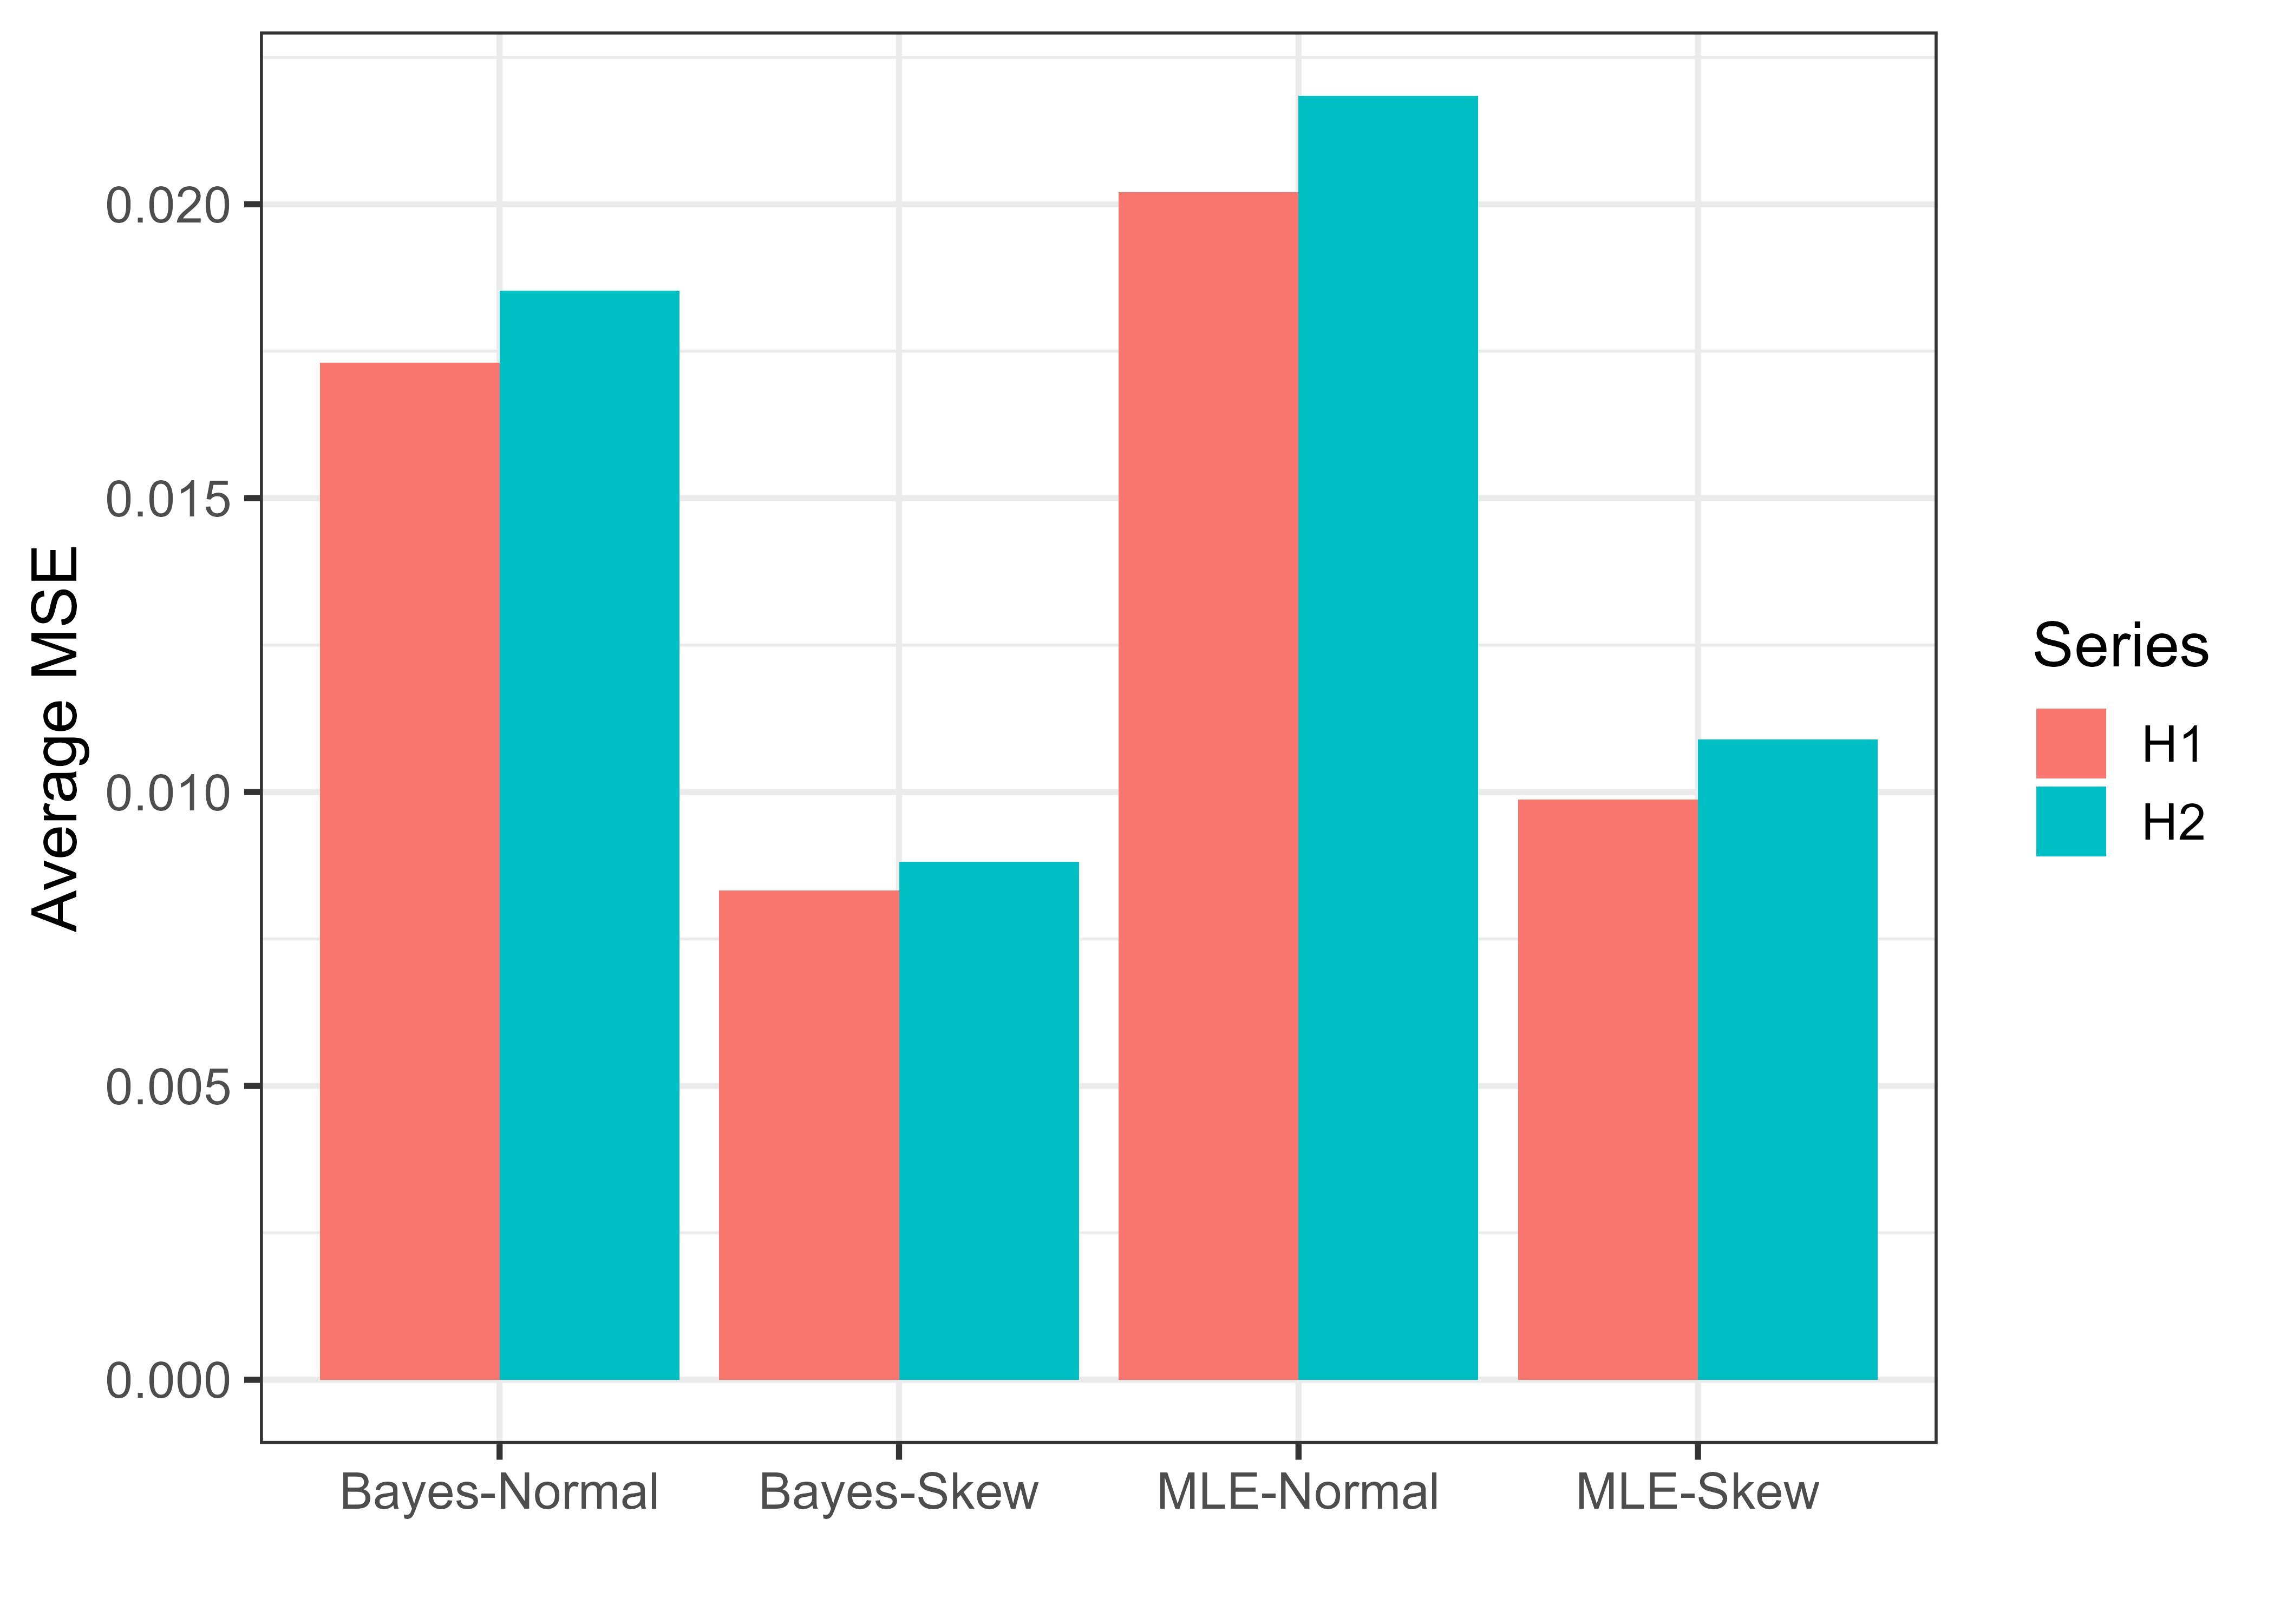
\includegraphics[width=.6\textwidth]{Scenario4_MeanMSE.png}
\caption{Average MSE of conditional volatility estimation under skew-normal innovations.}
\label{fig:MSE}
\end{figure}

To further quantify the practical importance of these differences, Figure~\ref{fig:Improve} reports the percentage reduction in MSE relative to the Gaussian maximum likelihood benchmark.

\begin{figure}[ht]
\centering
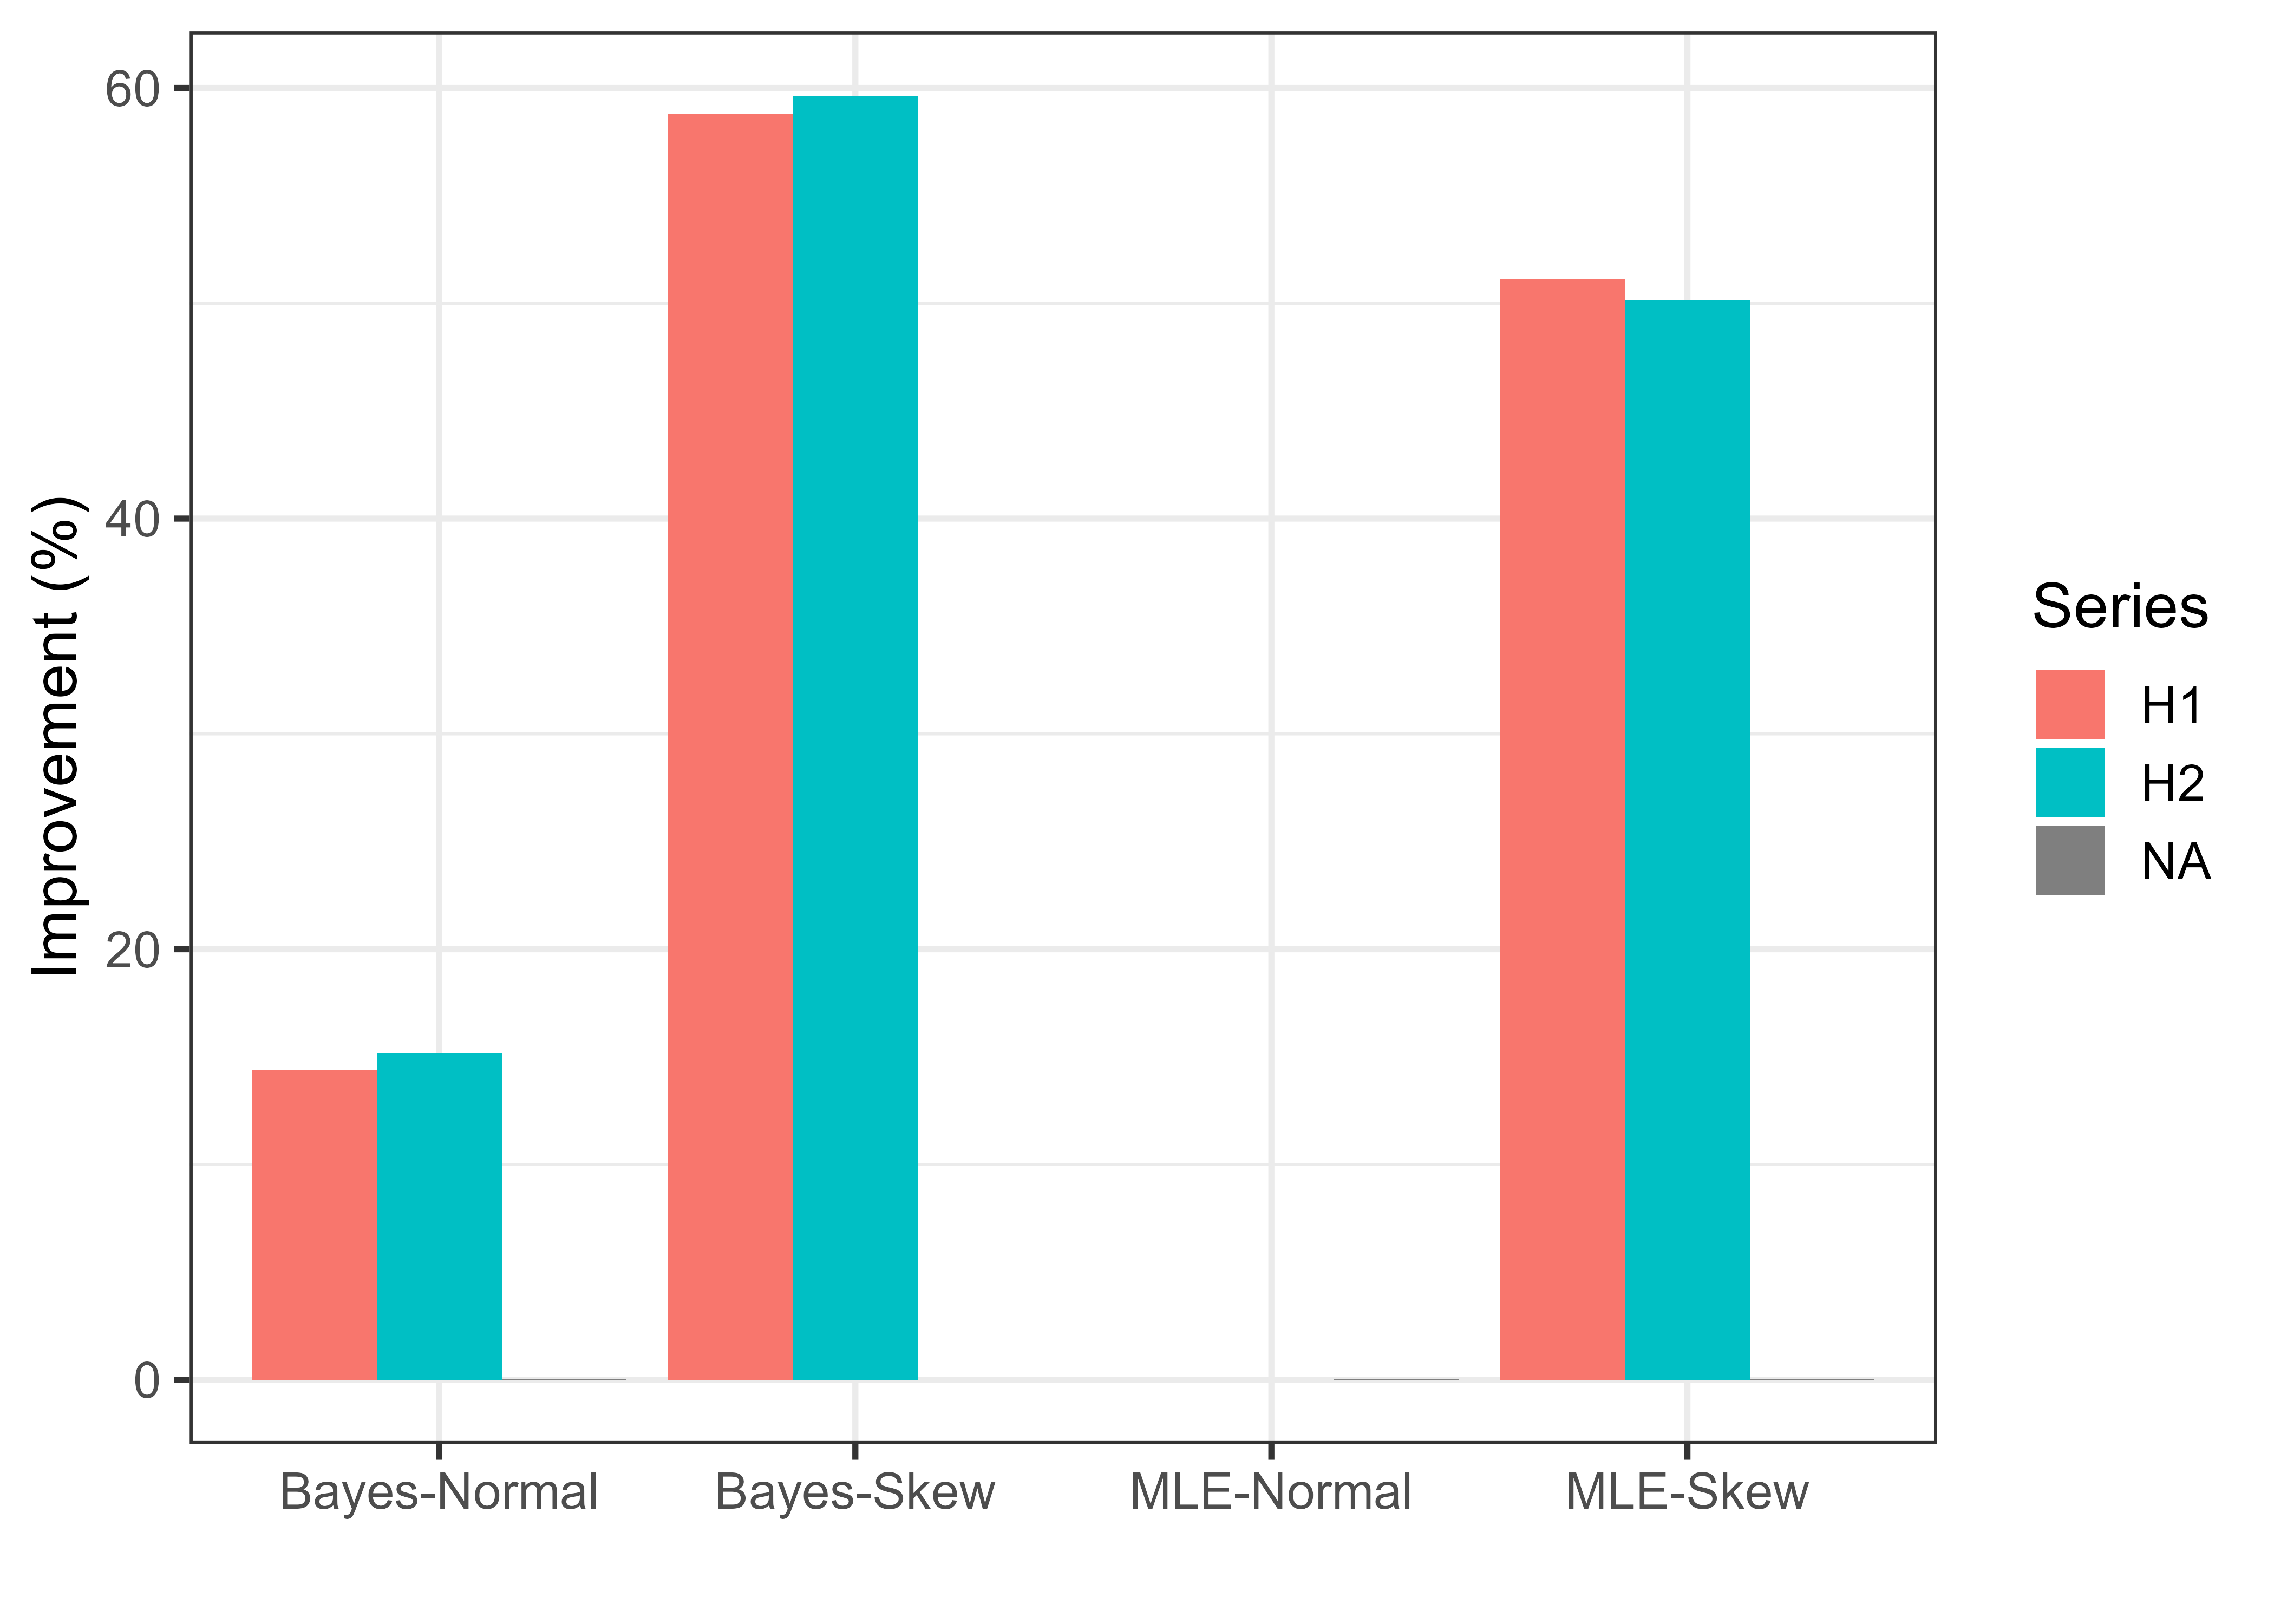
\includegraphics[width=.6\textwidth]{Scenario4_Improvement.png}
\caption{Percentage reduction in MSE relative to Gaussian MLE.}
\label{fig:Improve}
\end{figure}

The Bayes-Skew estimator achieves the best performance among all competing methods, reducing the volatility estimation error by approximately $59\%$ on average relative to the Gaussian maximum likelihood estimator. Overall, the simulation results indicate that correctly specifying the innovation distribution plays a crucial role in volatility estimation, while Bayesian inference provides additional efficiency gains by accounting for parameter uncertainty and improving the reconstruction of the latent volatility process.

\section*{Conclusion}

This paper proposes a Bayesian estimation framework for VAR-GoGARCH models under Gaussian and skew-normal innovations. The methodology combines Metropolis--Hastings sampling with the $\nu$SOBI algorithm to perform posterior inference in a computationally efficient manner.
Monte Carlo experiments show that the proposed Bayesian estimator consistently improves finite-sample estimation accuracy relative to maximum likelihood estimation. The results further indicate that accounting for asymmetric innovations plays an important role in volatility estimation. In particular, under skew-normal innovations, the Bayesian skew-normal specification achieves approximately a 59\% reduction in mean squared error compared with the Gaussian maximum likelihood benchmark.

Overall, the findings highlight the benefits of combining Bayesian inference with flexible innovation distributions for modeling multivariate financial time series with time-varying volatility.

Future research may extend the proposed framework to higher-dimensional systems and empirical financial applications.
\begin{thebibliography}{99}

\bibitem[Ardia and Hoogerheide (2010)]{Ardia2010}
Ardia, D. and Hoogerheide, L. (2010),
Bayesian estimation of the GARCH(1,1) model with Student-$t$ innovations,
\textit{The R Journal}, 2(2), 41--47.

\bibitem[Azzalini (1985)]{Azzalini1985}
Azzalini, A. (1985),
A class of distributions which includes the normal ones,
\textit{Scandinavian Journal of Statistics},12, 171--178.

\bibitem[Bollerslev (1986)]{Bollerslev1986}
Bollerslev, T. (1986),
Generalized autoregressive conditional heteroskedasticity,
\textit{Journal of Econometrics},
31(3), 307--327.

\bibitem[Engle (1982)]{Engle1982}
Engle, R. F. (1982),
Autoregressive conditional heteroscedasticity with estimates of the variance of United Kingdom inflation,
\textit{Econometrica: Journal of the econometric society}, 987--1007.

\bibitem[Miettinen et al. (2015)]{Miettinen2015}
Miettinen, M., Nordhausen, K., and Oja, H. (2015),
New independent component analysis tools for time series,
\textit{ Statistics \& Probability Letters},
105, 80--87.

\bibitem[Nakatsuma (2000)]{Nakatsuma2000}
Nakatsuma, T. (2000),
Bayesian analysis of ARMA-GARCH models: A Markov chain sampling approach,
\textit{Journal of Econometrics},
95(1), 57--69.

\bibitem[Van der Weide (2002)]{VanderWeide2002}
Van der Weide, R. (2002),
GO-GARCH: A multivariate generalized orthogonal GARCH model,
\textit{Journal of Applied Econometrics},
17(5), 549--564.


\bibitem[Virbickaitė et al. (2015)]{Virbickaite2016}
Virbickaite, A., Ausín, M.C. and Galeano, P. (2015),
BAYESIAN INFERENCE METHODS FOR UNIVARIATE AND MULTIVARIATE GARCH MODELS: A SURVEY,
\textit{Journal of Economic Surveys},
26, 76--96.

\end{thebibliography}

 \end{document}

